\documentclass{article}
\usepackage{ctex}
\usepackage{geometry}
\geometry{top = 2cm, left = 1cm, right = 1cm, bottom = 2cm}
\usepackage{amsmath,amssymb,amsthm,amsfonts}
\usepackage{abstract}
\usepackage{siunitx}
\usepackage{graphicx}

\title{用正比计数器测量X射线的吸收和特征谱}
\author{钱思天 2001112187}
\begin{document}
    \maketitle
    \begin{abstract}
        本实验利用了正比探测器和多道计数器,对经由$^{238}\text{Pu}$放射源激发的不同样品特征X射线进行了测量。通过对铁、钴、锗、铜、锌等元素的特征X射线测量,
        结合参考$K_\alpha$能谱对多道计数器进行了能量刻度。并利用刻度后的测量系统测量了三个未知样品的特征X射线能量,继而确定了元素种类。而后,通过添加不同厚度的
        铝吸收片的铜特征X射线的测量结果,测得了铝对X射线的线性吸收系数。最后,利用了$^{55}\text{Fe}$的特征X射线的测量结果,评估了正比探测器的分辨本领。
        \newline
        \newline
        {\emph{ 关键词:\ 正比计数器、特征X射线、线性吸收系数 }\rm}

    \end{abstract}

    \section{背景简介}
    \subsection{实验原理}
    \subsubsection{本征$X$射线谱}
    原子核通过核衰变过程(内转换及轨道电子俘获)或由外部射线激发而在其内层产生电子空穴,当外层电子向内层跃迁时发射的射线即为特征$X$射线。玻耳理论指出电子跃迁时放出的光子具有一定的波长$\lambda$它的能量为:
    \begin{equation}
        h v=Z^{2} \frac{2 \pi^{2} m_{0} e^{4}}{h^{2}}\left(\frac{1}{n_{1}^{2}}-\frac{1}{n_{2}^{2}}\right)
    \end{equation}
其中$n_1$、$n_2$为电子终态、始态所处壳层的主量子数,对$K_\alpha$线系
$n_1=1$,$n_2=2$。根据特征X射线的能量,可以辨认激发原子的原子序数。
    \subsubsection{$X$射线的吸收}
    $X$射线是一种能量较低的电磁波,它的波长在$100\text{\AA}$到$0.01\text{\AA}$之
间。当一束单色$X$射线垂直入射到某种材料上时,通过吸收体后的$X$射线强度将减弱,即$X$射线被物质吸收。它包含吸收和散射两个过程。
吸收过程主要包含光电吸收即光电效应。散射过程包含康普顿散射和汤姆逊散射。

设一厚度及成份均匀的吸收体,其厚度为$t$,每立方厘米有$N$个原子。若能量为$h\nu$的准直光束,单位时间内垂直入射到吸收体单位
面积上的光子数为$I_0$,那么通过厚度为$t$的物质后,透射出去的光子数为$I(t)$,并表示为:
\begin{equation}
    I(t) = I_0\exp(−\mu t) 
\end{equation}

式中$\mu$定义为线性吸收系数,$\mu=N\cdot\sigma$,$\sigma$为截面。

对于铝吸收材料,当$X$射线的能量低于$40\si{KeV}$时,光电效应占优势,康普顿散射可以忽略。光电效应的线性吸收系数为
\begin{equation}
    \mu_m = \frac{\mu}{\rho}(\si{cm^2\per g})=\phi_0 Z^5 \alpha^42^{5/2}(m_0c^2/h\nu)^{7/2}\frac{N_A}{A}
\end{equation}
式中,$\phi_0 = \frac{8}{3}\pi r_0^2, r_0 = \frac{e^2}{m_0c^2},\alpha\sim\frac{1}{137}$,而$N_A$是阿伏伽德罗常数,$A$是原子量。将铝元素代入,得
\begin{equation}
    \mu_m^{\text{Al}} = 52.694\si{cm^2\per g}
\end{equation}
\subsubsection{正比计数器}
正比计数器可将入射粒子(低能$\gamma$或$X$射线)产生的初电离效应
放大很多倍之后输出,并且输出信号的幅度仍然保持与初电离事件数目成正比,所以正比计数器不仅可以测量计数,还可以用来测量射线能量。由于正比计数管输出脉冲信号幅度比较大,而其本身噪声较小,
因此正比计数管可看成是一个没有噪声的理想放大器。这个特点决定了正比计数器在测量低能粒子方面有其独特的优势,广泛用于测量低
能$\gamma$射线和$X$射线的强度和能量。

正比计数器的能量分辨不仅受到由于原初电离的正负电荷对数
涨落的影响,还受气体放大倍数的影响,所以同样条件下,能量分辨要比$\text{Si}$($\text{Li}$)$X$射线谱仪差。
    \subsection{实验目的}
    \begin{enumerate}
        \item 学习使用正比计数器并熟悉其工作原理;
        \item 了解$X$射线与物质的相互作用原理、掌握其吸收规律;
        \item 利用元素特征$X$射线能量做探测器系统的刻度,并推断未知样品元素种类;
        \item 探测已知种类样品的特征$X$射线谱,评价实验探测系统的分辨率。
    \end{enumerate}
    \section{实验操作}
    \subsection{实验装置}
    实验装置示意图如图\ref{fig:ExpIns}。涉及的实验装置如下:
    \begin{figure}[htbp]
        \centering
        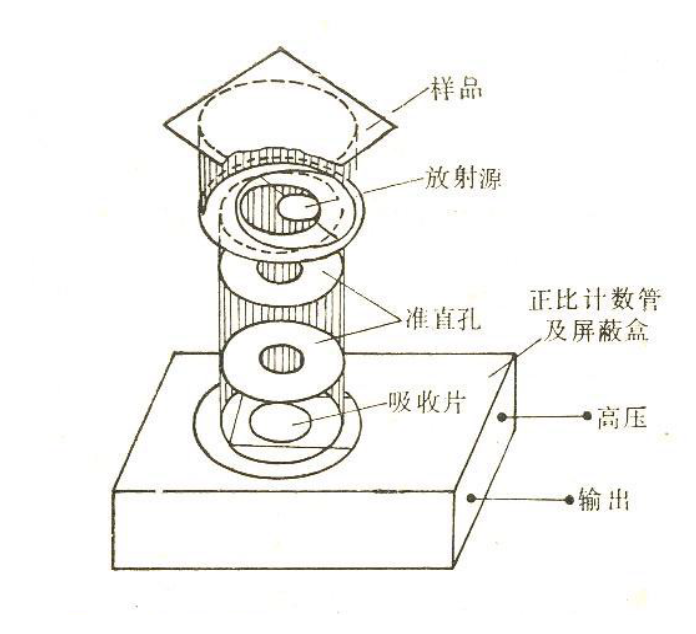
\includegraphics[width=0.5\textwidth]{../plot/ExpIns.png}
        \caption{实验装置示意图\label{fig:ExpIns}}
    \end{figure}
    \begin{enumerate}
        \item 正比计数器:一套;
        \item 电荷灵敏前置放大器(放大倍率:$\times 5$):一个;
        \item 插件式高压电源、低压电源、主放大器:各一个;
        \item NIM机箱:一个;
        \item 多道数据采集及微机系统:一套;
        \item 样品(铜等):若干;
        \item 铝吸收片:若干;
        \item $^{238}\text{Pu}$放射源:一枚;
        \item $^{55}\text{Fe}$放射源:一枚;
    \end{enumerate}
    \subsection{实验操作}
    \begin{enumerate}
        \item 观察已安装好的测量$X$射线的探头结构,连接仪器并预热(注
        意先开偏压,后加高压)。打开微机,进入微机多道数据采集系统。
        \item 逐渐升高正比计数器的高压至额定值约2000V,放大倍率设置为$0.9$倍。
        \item 用微机多道测量$^{238}\text{Pu}$源激发的五种已知样品的特征$X$射线谱(探测时间为$600\si{s}$)并
        确定其峰位。从附录特征$X$射线及吸收限表中查出各样品对应
        的$X$射线能量,作峰位道数-能量关系曲线。 
        \item 测量三个未知样品的特征$X$射线谱(探测时间为$600\si{s}$),根据能量刻度结果确定样
        品元素种类。
        \item 测量铜样品的特征$X$射线谱,并选定适当的阈值和道宽来确定
        峰面积计算范围。选择5个不同层数的铝吸收片(每片铝箔厚$2.15\si{mg\per cm^2}$),插在射线和探测器之间的插槽里,测量对应的铜样品的特征$X$射线强度(探测时间为$1200\si{s}$)。
        \item 对所测得的一组数据结果进行最小二乘法拟合,求出吸收系数$\mu_m$。
        \item 用微机多道对$^{55}\text{Fe}$源进行能谱测量,评价能量分辨率。
    \end{enumerate}
 

    \section{数据处理}
    
    \section{结论}
    
\end{document}